\section{Conexión con distintas teorías.}\label{seccion7}
\begin{center}
	\item \subsection{Teoría de grafos:}
\end{center}

\underline{\textbf{Definición:}}\\
Un \textbf{grafo} es un par $ (V,A) $ de conjuntos, junto con la aplicación 
\begin{center}
	 $  \gamma :A \rightarrow$ \{\{$u,v$\} / $u,v \in V$\}  
\end{center}
Al conjunto de puntos V se se llama conjunto de vértices y al conjunto A le llamaremos conjunto de aristas. \\

\underline{\textbf{Definición:}}\\
Un \textbf{grafo plano} $ G $ es un grafo que permanece en el plano.\\

Podemos ver varios ejemplos en la figura \ref{graf1}.\\
\begin{figure}[h!]
	\centering
	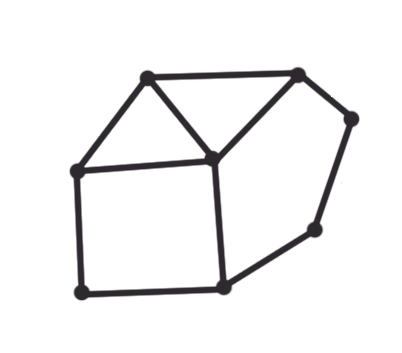
\includegraphics[width=3.5cm]{inudos/grafo.png}
	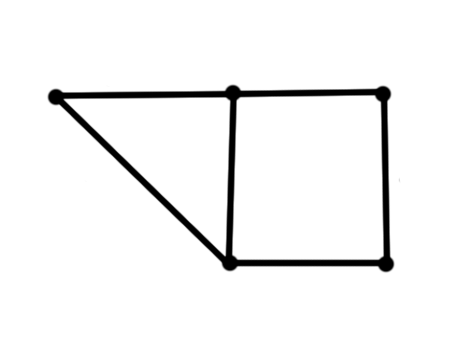
\includegraphics[width=4cm]{inudos/pgrafo.png}
	\caption{Ejemplos de grafos planos.}
	\label{graf1} 
\end{figure}

A partir de la proyección de un nudo (o de un enlace en general) podemos generar su grafo plano asociado. Para ello tendremos que realizar el siguiente proceso:\\

Sombreamos las regiones de la proyección que estén de modo que la región externa al nudo se quede sin sombrear y situamos un vértice en cada zona. Unimos los vértices con aristas que pasan por los cruces de la proyección. Ya tendríamos el grafo plano. Además, si el nudo tiene asignada una orientación, podremos asignarle el tipo de cruce (positivo o negativo) a cada arista. Podemos ver un ejemplo en la figura \ref{graf2}.\\
\begin{figure}[h!]
	\centering
	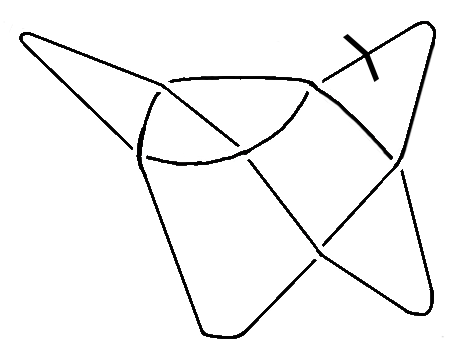
\includegraphics[width=5cm]{inudos/pgrafo3.png}
	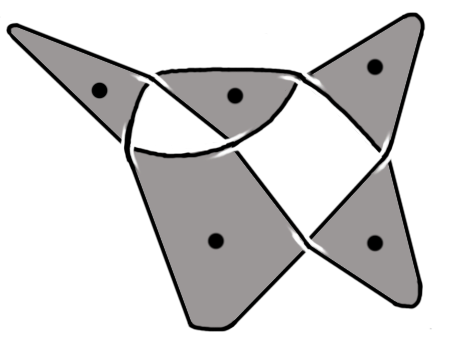
\includegraphics[width=5cm]{inudos/pgrafo2.png}
	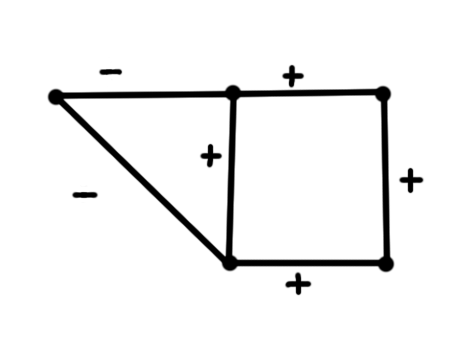
\includegraphics[width=5cm]{inudos/pgrafo1.png}
	\caption{De proyección a grafo}
	\label{graf2} 
\end{figure}

Finalmente, para ver que los problemas de nudos se pueden ver como problemas de grafos y viceversa, vamos a ver el procedimiento inverso. Dado un grafo plano, podremos obtener la proyección del nudo asociado. Veamos cuál sería el procedimiento:\\

Partiendo del grafo plano con los signos asociados en cada vértice, marcamos cada una de las aristas. Uniremos cada una de estas marcas con aquellas marcas que estén en las aristas que conectan con los vértices de la arista que tiene la marca. A continuación, sombreamos las zonas que contienen a cada vértice. Finalmente, establecemos los cruces conforme a los signos del grafo plano. Podemos ver un ejemplo en la figura \ref{graf3}.\\
\begin{figure}[h!]
	\centering
	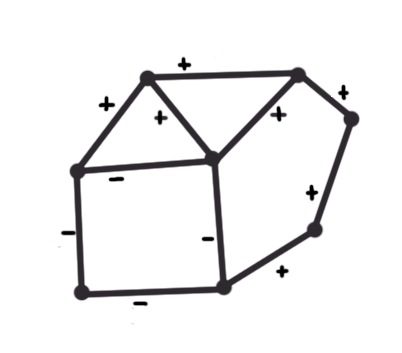
\includegraphics[width=4.5cm]{inudos/grafo1.png}
	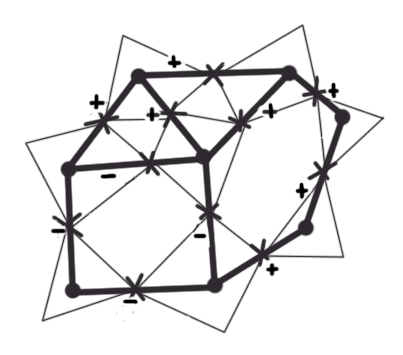
\includegraphics[width=4.5cm]{inudos/grafo2.png}
	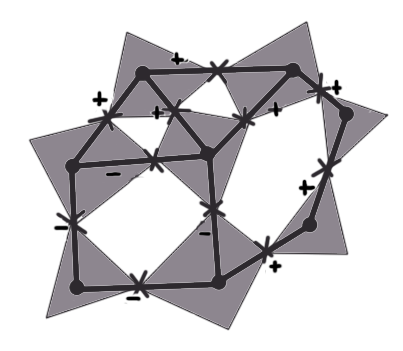
\includegraphics[width=4.5cm]{inudos/grafo3.png}
	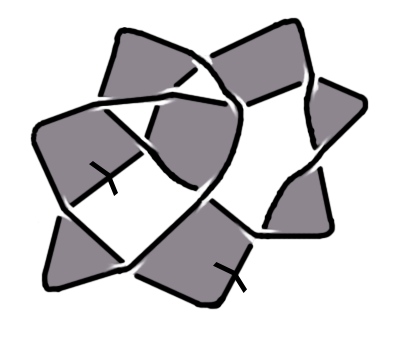
\includegraphics[width=4.5cm]{inudos/grafo4.png}
	\caption{De grafo a proyección.}
	\label{graf3} 
\end{figure}



\begin{center}
	\item \subsection{Teoría de trenzas:}
\end{center}
En esta sección vamos a introducir la relación que hay entre teoría de nudos y teoría de trenzas, teoría que estudiaremos con mayor detalle en el próximo tema.\\

Vamos a ver la idea general de lo que se entiende por el término trenza y veremos una definición más precisa más adelante. Podemos pensar en una trenza como un conjunto de $n$ cadenas que son atadas a un tope imaginario arriba y abajo. Podemos ver algunos ejemplos de trenzas en la figura \ref{ntren1}.\\
   \begin{figure}[h!]
   	\centering
   	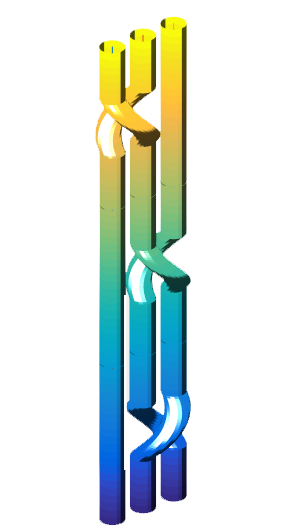
\includegraphics[width=3.5cm]{itrenzas/t4.png}
   	\space
   	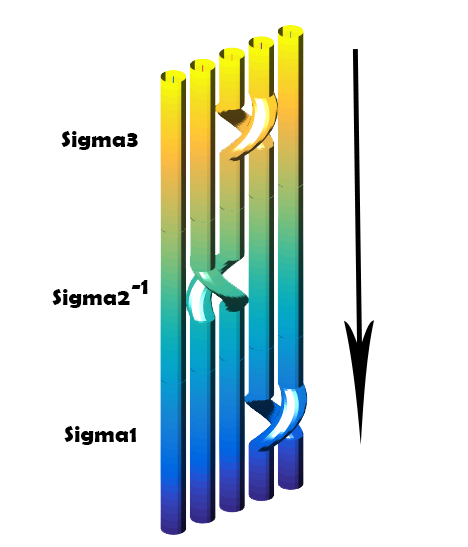
\includegraphics[width=6cm]{itrenzas/t7.png}
   	\caption{Ejemplos de trenzas}
   	\label{ntren1} 
   \end{figure} 

A partir de una trenza, podemos obtener su nudo o enlace correspondiente. Simplemente tendremos que unir en orden  los topes superiores de las cadenas con los inferiores. Esta trenza cerrada será el nudo al que representa la trenza. Podemos ver algunos ejemplos en la sección \ref{t2sec1}.\\

Para ver el proceso inverso haremos uso del siguiente teorema:
\begin{teo}Teorema de Alexander.\\
	Todo nudo puede ser representado como una trenza cerrada.
\end{teo}

Para ver la demostración de dicho teorema podemos inspirarnos en varias ideas \cite{13}, \cite{14}. En este caso vamos a ver el algoritmo de Yamada-Vogel, que transforma un nudo en una trenza cerrada. Este proceso se puede realizar a cualquier nudo y el resultado es siempre una trenza cerrada. 
\begin{proof}
	Dada nudo orientado K, realizaremos los siguientes pasos:
	\begin{enumerate}
		\item A partir de la proyección D del nudo K, vamos a obtener su imagen de Seifert S realizando el siguiente proceso:\\
		Sabemos que en cada cruce de la proyección D nos encontramos dos hebras entrando al cruce y dos hebras salientes. Vamos a eliminar el cruce conectando cada una de las hebras que entran al cruce con las hebras adyacentes que salen del mismo. Podemos ver la idea en la figura \ref{prueale1}.\\
		
		\begin{figure}[h!]
			\centering
			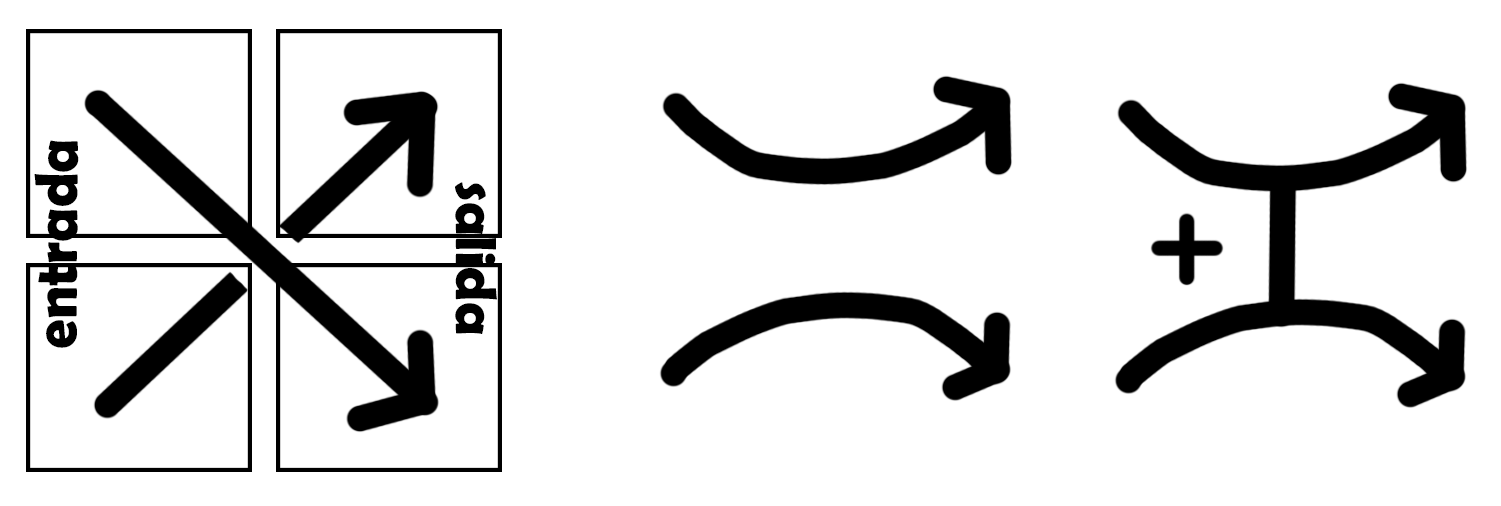
\includegraphics[width=12cm]{inudos/ima8.png}
			\caption{Transformando la proyección de un cruce.}
			\label{prueale1} 
		\end{figure}
		
		
		Como resultado, vamos a obtener un conjunto de círculos en el plano a los que se les conoce como círculos de Seifert. \\
		Para no perder el tipo de cruce, vamos a conservar la conexión de los cruces y asignaremos el símbolo + a los cruces positivos y el símbolo - a los cruces negativos. De este modo, conseguimos conservar toda la información sobre la proyección del nudo. 
		
		\item Antes de ver cómo realizar este segundo paso, necesitamos unos conceptos previos. \\
	
		Sean dos círculos de Seifert C1 y C2. Diremos que son incoherentes si no existe un arco que los conecte.\\
		Definimos la altura de la proyección D (h(D)) como el número de pares de círculos de Seifert incoherentes.\\
		
		Si h(D)=0, entonces D ya representa una trenza cerrada, finalizo.\\
		Si h(D)$ > $0, podemos encontrar un arco que una dos pares de círculos de Seifert incoherentes (se conoce como arco de reducción). Se puede de ver cómo representaremos un arco de reducción entre dos círculos de Seifert en la figura \ref{prueale2}.
		\begin{figure}[h!]
			\centering
			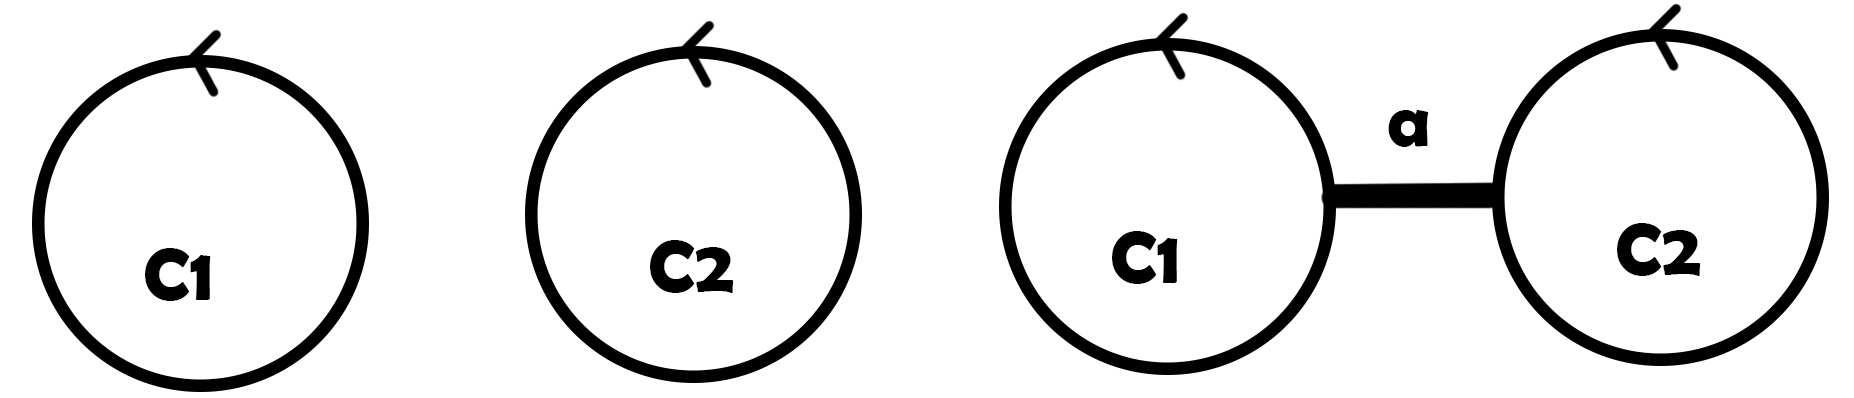
\includegraphics[width=11cm]{inudos/ima10.png}
			\caption{Arco de reducción.}
			\label{prueale2} 
		\end{figure}
		
		 Este arco de reducción nos sirve de guía para realizar un movimiento de reducción sobre ambos círculos de Seifert de modo que obtenemos la primera proyección de la figura \ref{prueale3}. Con las siguientes imágenes de la figura vemos que efectivamente se conservan los círulos de Seifert originales pero hemos conseguido que ahora sean coherentes. 
		\begin{figure}[h!]
			\centering
			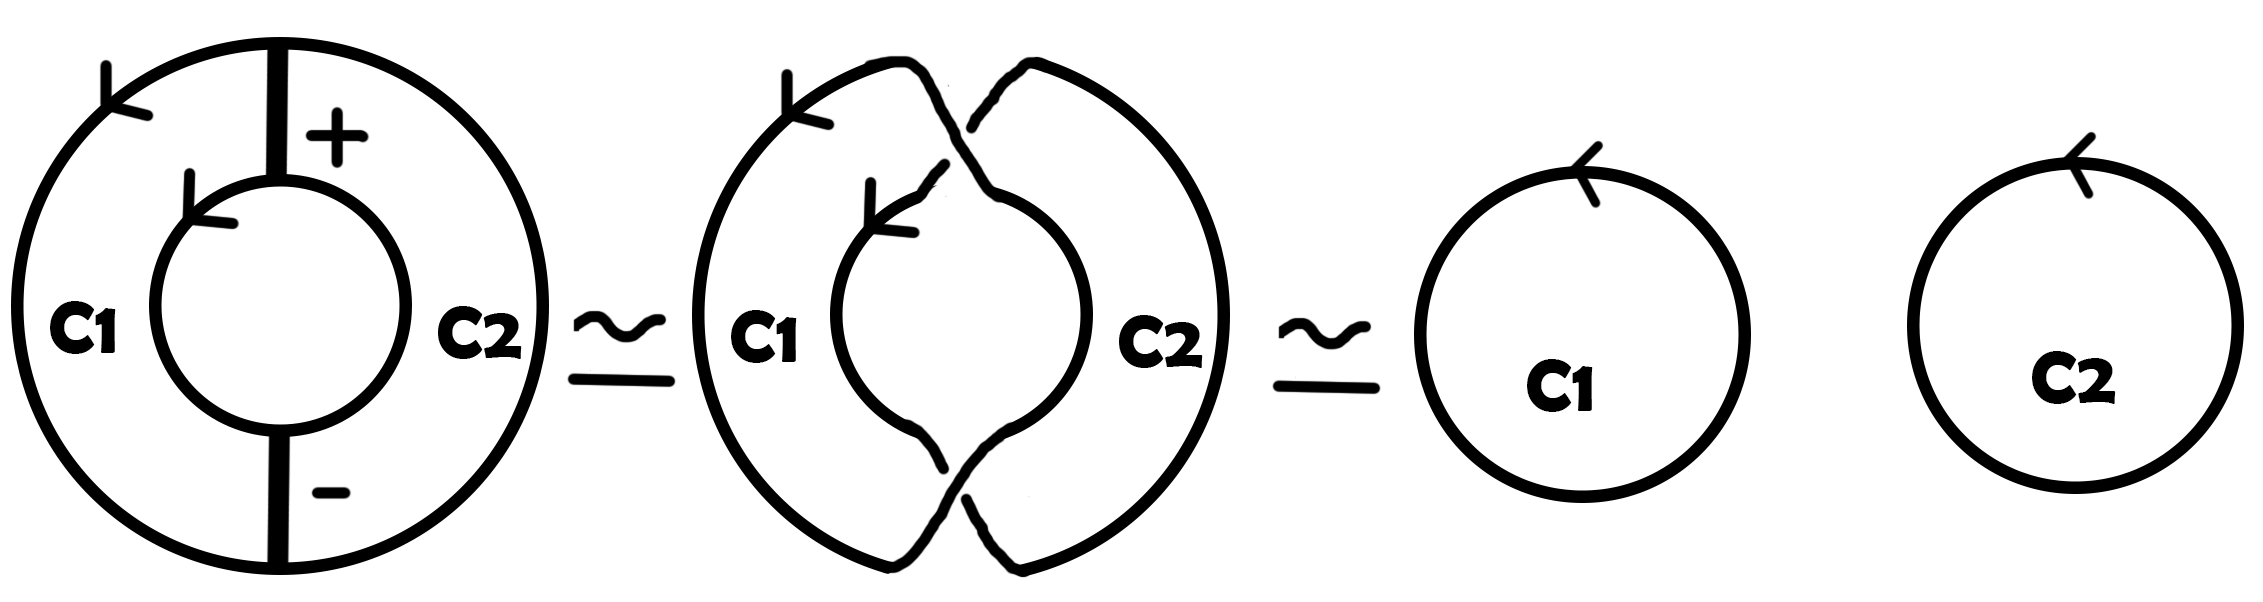
\includegraphics[width=13cm]{inudos/ima11.png}
			\caption{Movimiento de reducción.}
			\label{prueale3} 
		\end{figure}
	
		
		\item Continuamos realizando movimientos de reducción hasta obtener h(D)=0.\\
		
		Se puede demostrar \cite{13} que dicho algoritmo finaliza haciendo uso del siguiente lema:\\
		Supongamos que realizamos un movimiento de reducción al a proyección D, obteniendo la proyección D'. En ese caso, h(D')=h(D)-1.
		
	\end{enumerate}
\end{proof} 

En la figura \ref{prueale4} aplicamos el algoritmo a un nudo particular. 
		\begin{figure}[h!]
			\centering
			\subfigure[Proyección nudo]{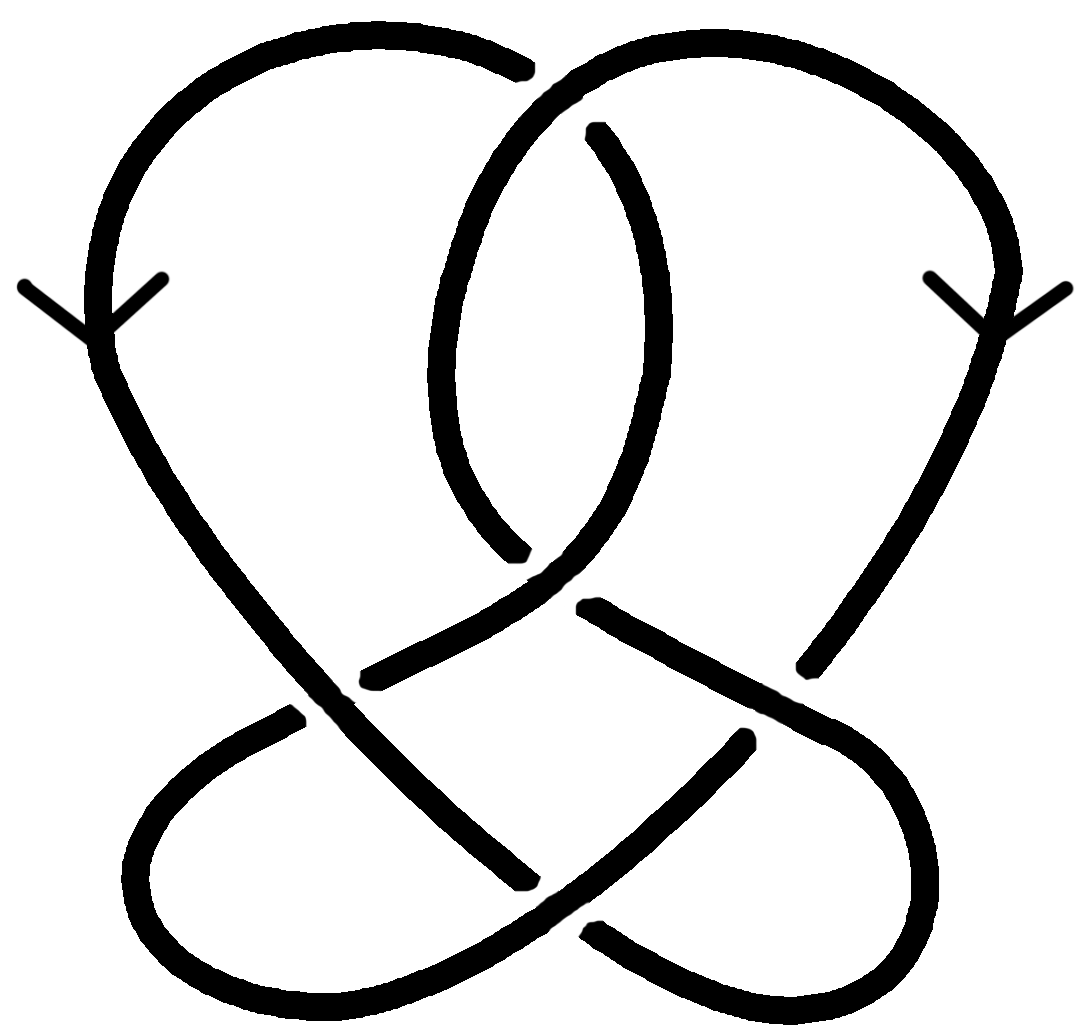
\includegraphics[width=4.5cm]{inudos/ima1.png}}
			\subfigure[Círculos Seifert]{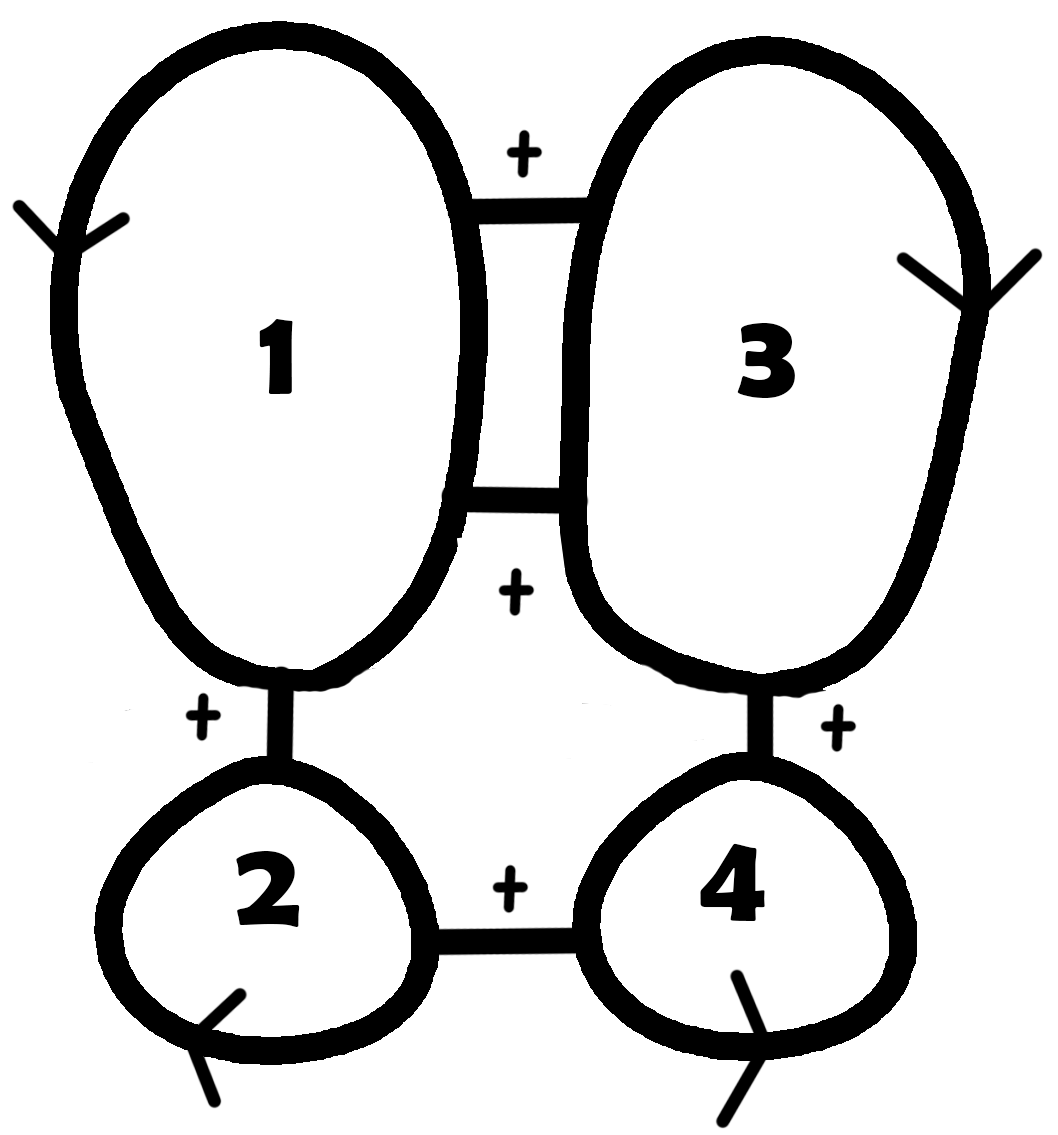
\includegraphics[width=4cm]{inudos/ima3.png}}
			\caption{Movimiento de reducción.}		
			\subfigure[Círculos Seifert]{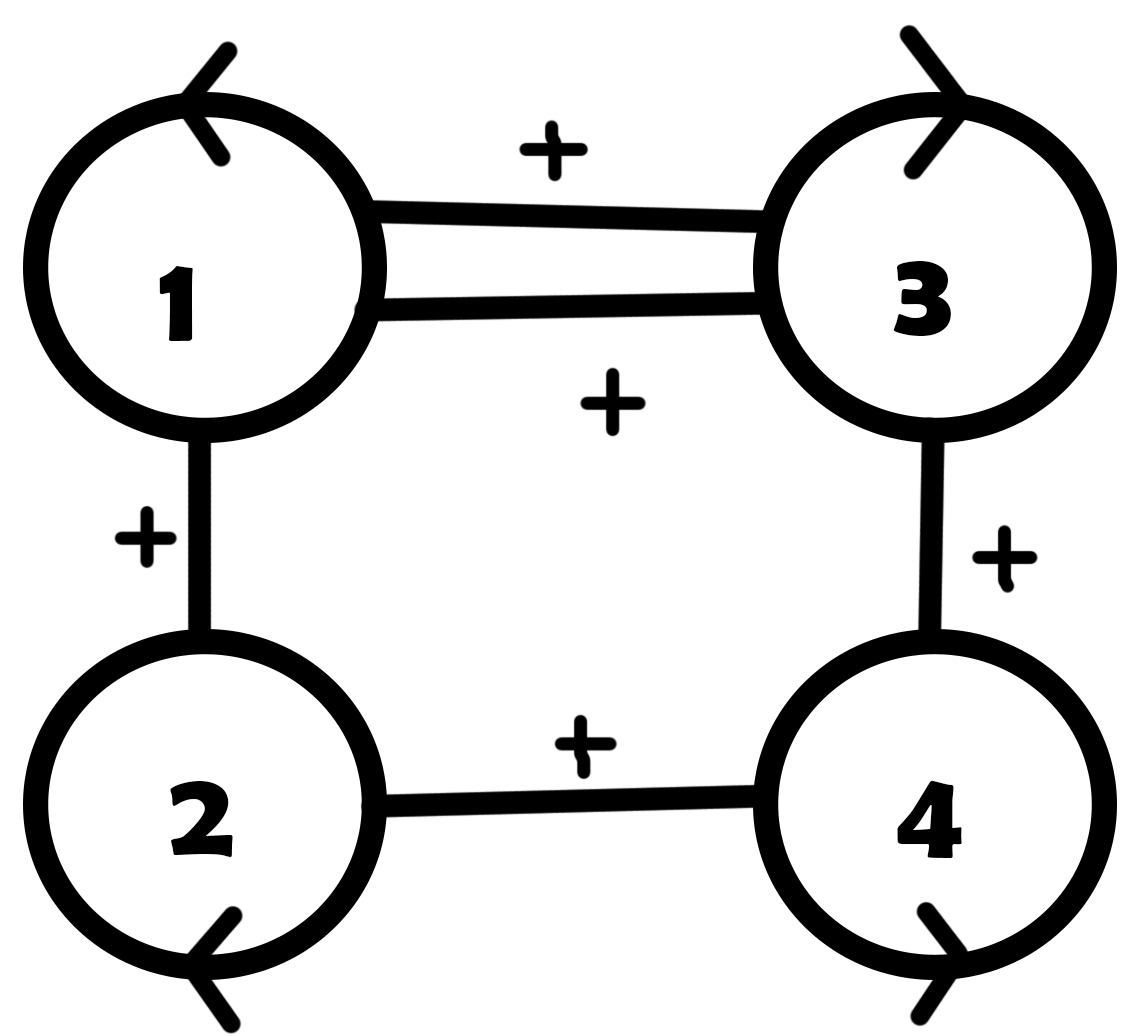
\includegraphics[width=4cm]{inudos/ima4.png}}
			\subfigure[Arco reducción]{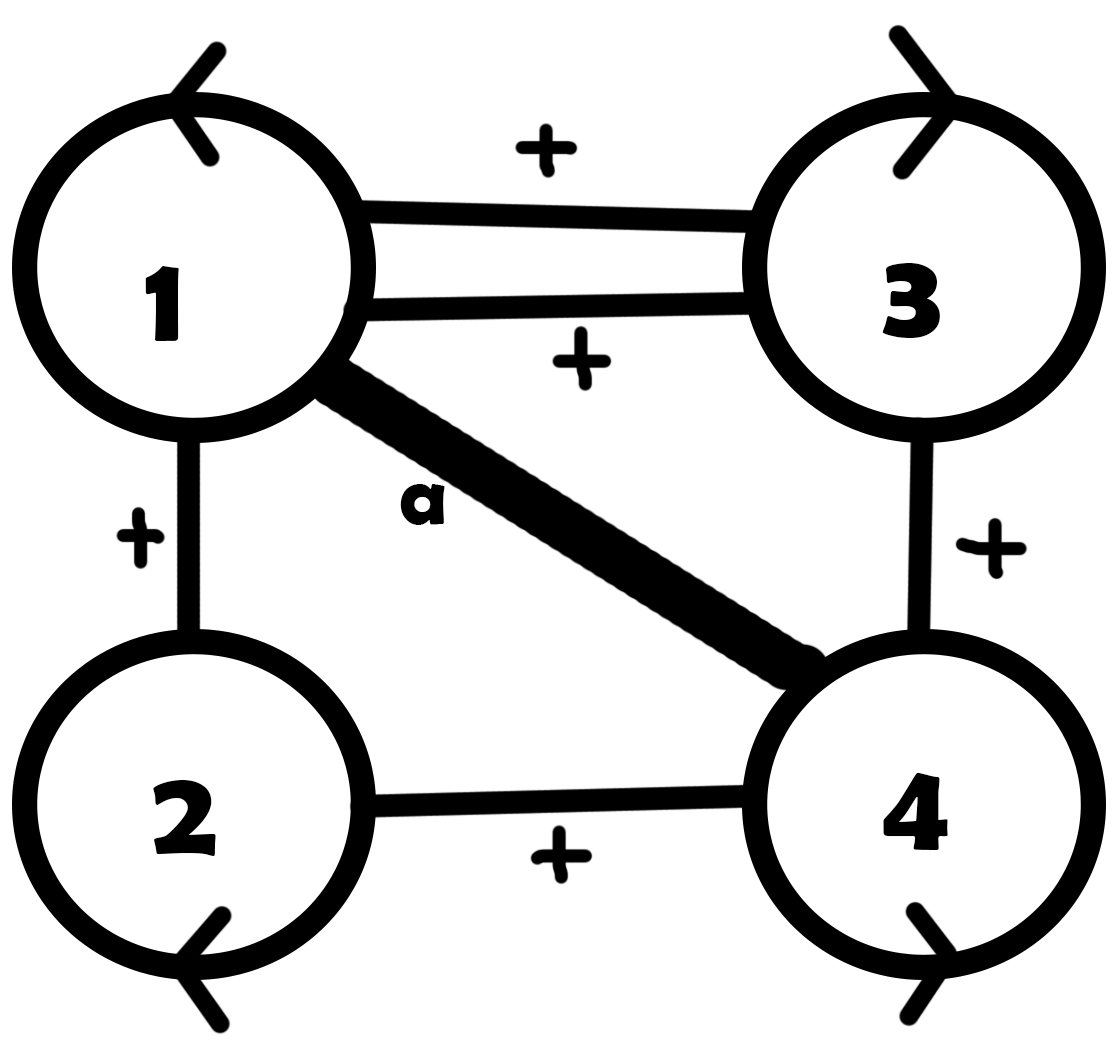
\includegraphics[width=4cm]{inudos/ima5.png}}
			
			\subfigure[Movimiento reducción]{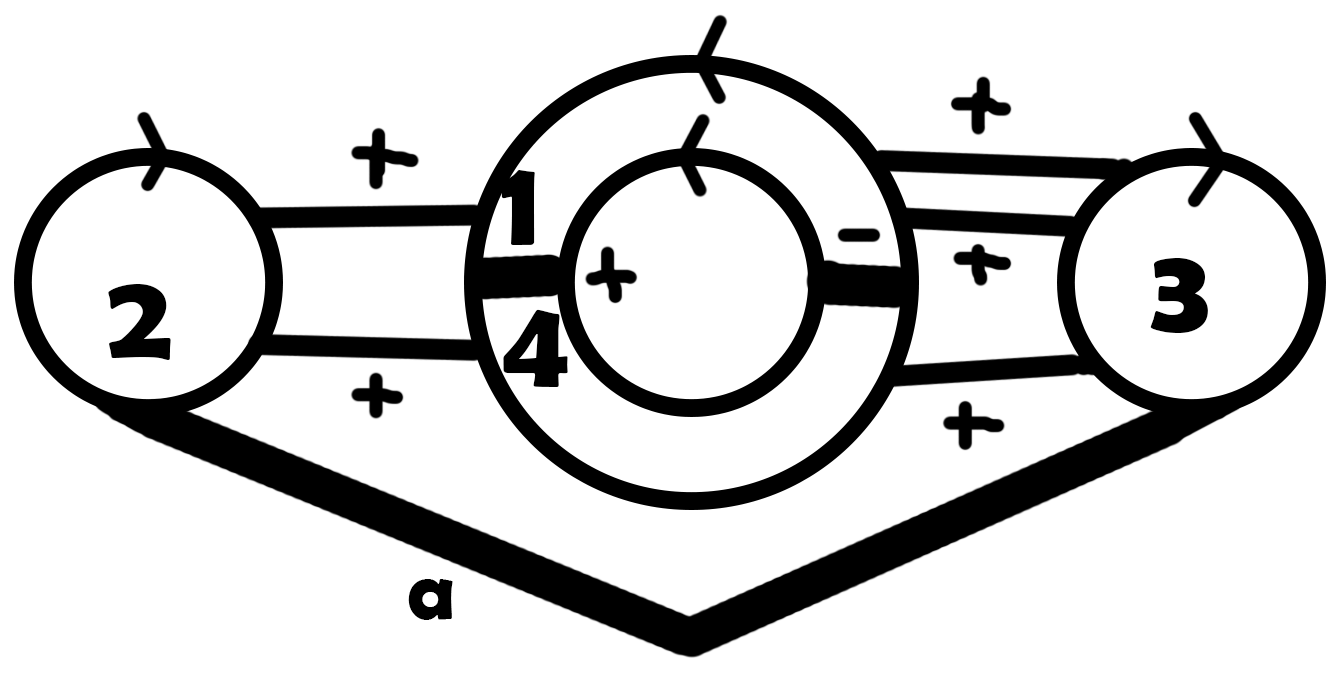
\includegraphics[width=7.8cm]{inudos/ima6.png}}
			\subfigure[Movimiento reducción]{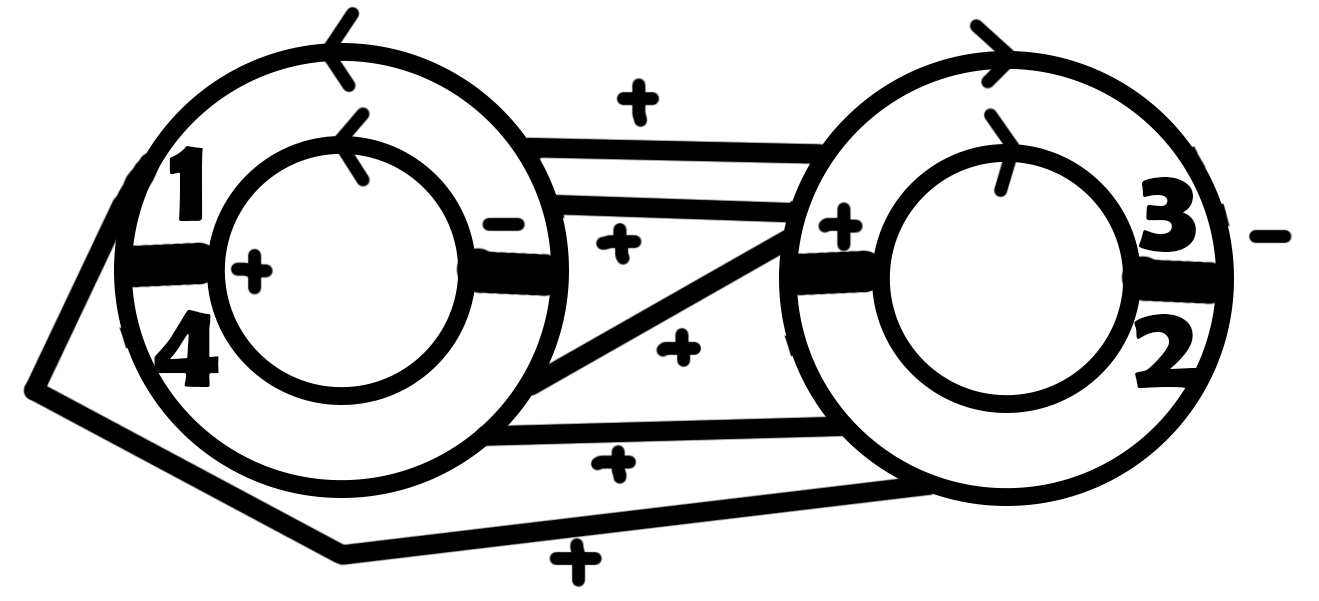
\includegraphics[width=7.8cm]{inudos/ima7.png}}
			\subfigure[Final]{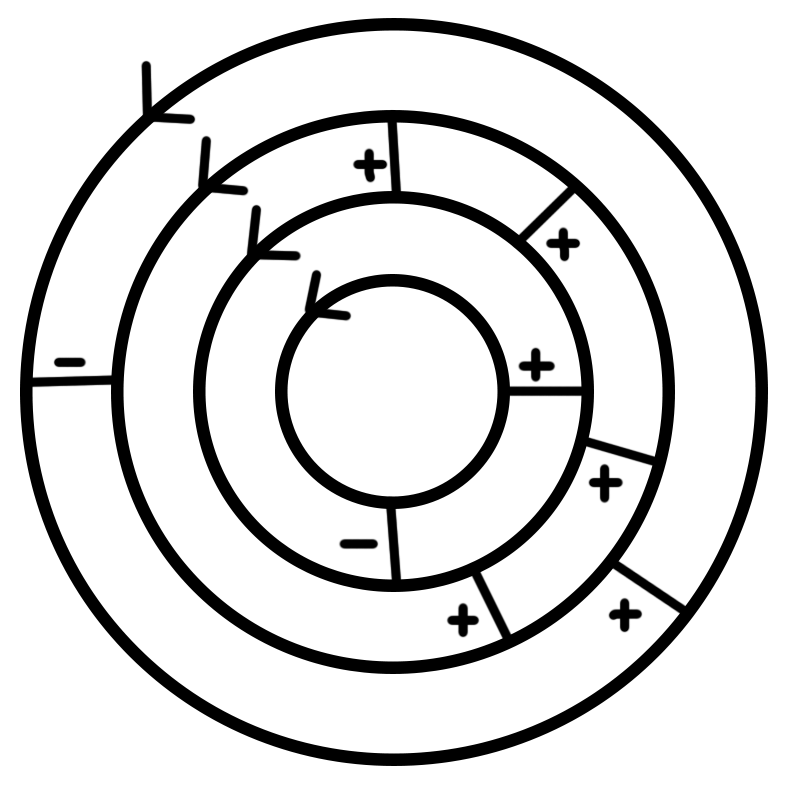
\includegraphics[width=4.5cm]{inudos/ima9.png}}
			\caption{Movimiento de reducción.}
			\label{prueale4} 
		\end{figure}
